\documentclass[12pt,a4paper]{article}
\usepackage[utf8]{inputenc}
\usepackage[margin=1in]{geometry}
\usepackage{graphicx}
\usepackage{hyperref}
\usepackage{listings}
\usepackage{xcolor}
\usepackage{tikz}
\usepackage{enumitem}
\usepackage{fancyhdr}
\usepackage{tcolorbox}
\usepackage{amsmath}
\usepackage{booktabs}
\usepackage{longtable}

% Code styling
\definecolor{codegreen}{rgb}{0,0.6,0}
\definecolor{codegray}{rgb}{0.5,0.5,0.5}
\definecolor{codepurple}{rgb}{0.58,0,0.82}
\definecolor{backcolour}{rgb}{0.95,0.95,0.92}

\lstdefinestyle{mystyle}{
    backgroundcolor=\color{backcolour},   
    commentstyle=\color{codegreen},
    keywordstyle=\color{magenta},
    numberstyle=\tiny\color{codegray},
    stringstyle=\color{codepurple},
    basicstyle=\ttfamily\footnotesize,
    breakatwhitespace=false,         
    breaklines=true,                 
    captionpos=b,                    
    keepspaces=true,                 
    numbers=left,                    
    numbersep=5pt,                  
    showspaces=false,                
    showstringspaces=false,
    showtabs=false,                  
    tabsize=2
}

\lstset{style=mystyle}

% Header and Footer
\pagestyle{fancy}
\fancyhf{}
\rhead{ITC Inventory Management System}
\lhead{Technical Documentation}
\cfoot{\thepage}

\title{\textbf{ITC Warehouse Inventory Management System} \\ \Large{Complete Technical Documentation}}
\author{Priyanshu \\ \texttt{priyansh85953@gmail.com}}
\date{\today}

\begin{document}

\maketitle
\thispagestyle{empty}

\begin{center}
\large
\textbf{Version:} 1.0.0 \\
\textbf{Deployment:} Azure Web App (Central India) \\
\textbf{Live URL:} \href{https://itc-warehouse-app-2025-c8hgg5deeagae5dj.centralindia-01.azurewebsites.net}{ITC Warehouse App}
\end{center}

\newpage
\tableofcontents
\newpage

%===============================================
\section{Executive Summary}
%===============================================

The ITC Warehouse Inventory Management System is a full-stack web application designed to streamline warehouse operations for ITC Limited. The system manages inventory tracking, bin assignments, incoming/outgoing operations, and provides real-time monitoring capabilities for supervisors.

\subsection{Key Features}
\begin{itemize}
    \item \textbf{Real-time Inventory Tracking} with FIFO (First-In-First-Out) logic
    \item \textbf{QR Code-based Operations} for bin scanning and verification
    \item \textbf{Role-based Access Control} (Operators and Supervisors)
    \item \textbf{Auto Weight Calculation} using SKU master data ($Weight = CFC \times UOM$)
    \item \textbf{Task Monitoring System} with 30-minute timeout protection
    \item \textbf{Active SKU Management} for inventory control
    \item \textbf{Comprehensive Reporting} and analytics dashboard
\end{itemize}

%===============================================
\section{System Architecture}
%===============================================

\subsection{Technology Stack}

\begin{tcolorbox}[colback=blue!5!white,colframe=blue!75!black,title=Full Stack Architecture]
\begin{itemize}[leftmargin=*]
    \item \textbf{Frontend:} Vanilla JavaScript, HTML5, CSS3
    \item \textbf{Backend:} Node.js (v18+) with Express.js framework
    \item \textbf{Database:} PostgreSQL 13+ (Azure Flexible Server)
    \item \textbf{Deployment:} Azure App Service (Linux, Node 22-lts)
    \item \textbf{Version Control:} Git/GitHub with CI/CD
    \item \textbf{QR Generation:} qrcode npm library (v1.5.3)
\end{itemize}
\end{tcolorbox}

\subsection{Architecture Diagram}

\begin{center}
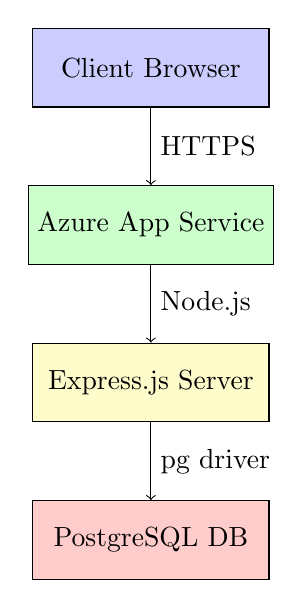
\begin{tikzpicture}[node distance=2cm]
    % Nodes
    \node (client) [draw, rectangle, fill=blue!20, minimum width=3cm, minimum height=1cm] {Client Browser};
    \node (azure) [draw, rectangle, fill=green!20, below of=client, minimum width=3cm, minimum height=1cm] {Azure App Service};
    \node (express) [draw, rectangle, fill=yellow!20, below of=azure, minimum width=3cm, minimum height=1cm] {Express.js Server};
    \node (postgres) [draw, rectangle, fill=red!20, below of=express, minimum width=3cm, minimum height=1cm] {PostgreSQL DB};
    
    % Arrows
    \draw[->] (client) -- node[right] {HTTPS} (azure);
    \draw[->] (azure) -- node[right] {Node.js} (express);
    \draw[->] (express) -- node[right] {pg driver} (postgres);
\end{tikzpicture}
\end{center}

%===============================================
\section{Database Design}
%===============================================

\subsection{Database Platform: PostgreSQL}

\textbf{Why PostgreSQL?}
\begin{itemize}
    \item ACID compliance for transaction integrity
    \item Excellent support for complex queries and joins
    \item JSON/JSONB support for flexible data storage
    \item Azure Flexible Server provides managed hosting
    \item High concurrency support for multiple operators
\end{itemize}

\textbf{Connection Details:}
\begin{lstlisting}[language=bash]
Host: itc-warehouse-db-2025.postgres.database.azure.com
Port: 5432
Database: itc_warehouse
User: itcadmin
SSL: Required (Azure enforced)
\end{lstlisting}

\subsection{Database Schema}

\subsubsection{Core Tables}

\paragraph{1. Inventory Table}
\begin{tcolorbox}[colback=gray!5!white,colframe=gray!75!black]
\textbf{Purpose:} Real-time inventory tracking with bin-SKU relationships

\begin{lstlisting}[language=SQL]
CREATE TABLE "Inventory" (
    id SERIAL PRIMARY KEY,
    bin_no VARCHAR(10) NOT NULL,
    sku VARCHAR(50) NOT NULL,
    batch_no VARCHAR(50),
    cfc INTEGER DEFAULT 0,
    description TEXT,
    uom DECIMAL(10,3),
    created_at TIMESTAMP DEFAULT CURRENT_TIMESTAMP,
    updated_at TIMESTAMP DEFAULT CURRENT_TIMESTAMP,
    UNIQUE(bin_no, sku)
);
\end{lstlisting}

\textbf{Key Features:}
\begin{itemize}
    \item Composite unique constraint on (bin\_no, sku)
    \item Auto-updated timestamps for audit trail
    \item CFC (Case Full Carton) tracking
    \item UOM (Unit of Measure) for weight calculations
\end{itemize}
\end{tcolorbox}

\paragraph{2. Bins Table}
\begin{tcolorbox}[colback=gray!5!white,colframe=gray!75!black]
\textbf{Purpose:} Physical bin master data

\begin{lstlisting}[language=SQL]
CREATE TABLE "Bins" (
    id SERIAL PRIMARY KEY,
    bin_no VARCHAR(10) UNIQUE NOT NULL,
    location VARCHAR(100),
    capacity INTEGER DEFAULT 50,
    current_sku VARCHAR(50),
    current_qty INTEGER DEFAULT 0,
    status VARCHAR(20) DEFAULT 'empty',
    created_at TIMESTAMP DEFAULT CURRENT_TIMESTAMP
);
\end{lstlisting}

\textbf{Status Values:}
\begin{itemize}
    \item \texttt{empty}: No inventory
    \item \texttt{partial}: Partially filled
    \item \texttt{full}: At capacity
\end{itemize}
\end{tcolorbox}

\paragraph{3. Cleaned\_FG\_Master\_file Table}
\begin{tcolorbox}[colback=gray!5!white,colframe=gray!75!black]
\textbf{Purpose:} SKU master data repository

\begin{lstlisting}[language=SQL]
CREATE TABLE "Cleaned_FG_Master_file" (
    sku VARCHAR(50) PRIMARY KEY,
    description TEXT,
    uom DECIMAL(10,3),
    created_at TIMESTAMP DEFAULT CURRENT_TIMESTAMP
);
\end{lstlisting}

\textbf{Usage:}
\begin{itemize}
    \item Source of truth for SKU information
    \item UOM values used for weight calculation: $Weight = CFC \times UOM$
    \item Example: FXC10005PB has UOM = 2.520 kg/CFC
\end{itemize}
\end{tcolorbox}

\paragraph{4. Operators Table}
\begin{tcolorbox}[colback=gray!5!white,colframe=gray!75!black]
\textbf{Purpose:} User authentication and role management

\begin{lstlisting}[language=SQL]
CREATE TABLE "Operators" (
    id SERIAL PRIMARY KEY,
    operator_id VARCHAR(50) UNIQUE NOT NULL,
    name VARCHAR(100),
    email VARCHAR(100) UNIQUE,
    password VARCHAR(255),
    role VARCHAR(20) DEFAULT 'operator',
    created_at TIMESTAMP DEFAULT CURRENT_TIMESTAMP
);
\end{lstlisting}

\textbf{Roles:}
\begin{itemize}
    \item \texttt{operator}: Standard warehouse operator
    \item \texttt{supervisor}: Manager with monitoring capabilities
\end{itemize}
\end{tcolorbox}

\paragraph{5. Task\_History Table}
\begin{tcolorbox}[colback=gray!5!white,colframe=gray!75!black]
\textbf{Purpose:} Audit trail for all warehouse operations

\begin{lstlisting}[language=SQL]
CREATE TABLE "Task_History" (
    id SERIAL PRIMARY KEY,
    session_token VARCHAR(255),
    operator VARCHAR(100),
    task_type VARCHAR(20),
    sku VARCHAR(50),
    quantity INTEGER,
    bins_used TEXT,
    status VARCHAR(20) DEFAULT 'pending',
    started_at TIMESTAMP,
    completed_at TIMESTAMP,
    duration_minutes INTEGER,
    cancelled_at TIMESTAMP,
    cancellation_reason TEXT,
    created_at TIMESTAMP DEFAULT CURRENT_TIMESTAMP
);
\end{lstlisting}

\textbf{Task Types:}
\begin{itemize}
    \item \texttt{incoming}: Inventory receipt operations
    \item \texttt{outgoing}: Dispatch/picking operations
\end{itemize}
\end{tcolorbox}

\paragraph{6. active\_skus Table}
\begin{tcolorbox}[colback=gray!5!white,colframe=gray!75!black]
\textbf{Purpose:} Dynamic SKU filtering for operators

\begin{lstlisting}[language=SQL]
CREATE TABLE IF NOT EXISTS active_skus (
    id SERIAL PRIMARY KEY,
    sku VARCHAR(50) UNIQUE NOT NULL,
    is_active BOOLEAN DEFAULT true,
    created_at TIMESTAMP DEFAULT CURRENT_TIMESTAMP,
    updated_at TIMESTAMP DEFAULT CURRENT_TIMESTAMP
);
\end{lstlisting}

\textbf{Functionality:}
\begin{itemize}
    \item Supervisors control which SKUs operators can access
    \item Reduces operator confusion with focused SKU list
    \item Real-time updates via supervisor dashboard
\end{itemize}
\end{tcolorbox}

\paragraph{7. user\_sessions Table}
\begin{tcolorbox}[colback=gray!5!white,colframe=gray!75!black]
\textbf{Purpose:} Session management and authentication tokens

\begin{lstlisting}[language=SQL]
CREATE TABLE IF NOT EXISTS user_sessions (
    id SERIAL PRIMARY KEY,
    session_token VARCHAR(255) UNIQUE NOT NULL,
    operator_id VARCHAR(50),
    email VARCHAR(100),
    name VARCHAR(100),
    role VARCHAR(20),
    created_at TIMESTAMP DEFAULT CURRENT_TIMESTAMP,
    expires_at TIMESTAMP,
    is_active BOOLEAN DEFAULT true
);
\end{lstlisting}

\textbf{Security Features:}
\begin{itemize}
    \item Token-based authentication (not cookie-based)
    \item Automatic expiration handling
    \item Active session tracking
\end{itemize}
\end{tcolorbox}

\subsubsection{Additional Tables}

\begin{itemize}
    \item \textbf{Incoming}: Tracks incoming inventory transactions
    \item \textbf{Outgoing}: Tracks outgoing dispatch transactions
    \item \textbf{Historical\_Log}: Archive table for old records
\end{itemize}

%===============================================
\section{Backend Architecture (Node.js + Express)}
%===============================================

\subsection{Server Configuration}

\textbf{Entry Point:} \texttt{server.js} (2751 lines)

\begin{lstlisting}[language=JavaScript]
const express = require('express');
const cors = require('cors');
const db = require('./database/db');
const QRCode = require('qrcode');
const dotenv = require('dotenv');

dotenv.config();

const app = express();
const PORT = process.env.PORT || 3000;

// Middleware
app.use(cors());
app.use(express.json());
app.use(express.static('public'));

// Start server
app.listen(PORT, () => {
    console.log(`Server running on port ${PORT}`);
});
\end{lstlisting}

\subsection{Database Connection Module}

\textbf{File:} \texttt{database/db.js}

\begin{lstlisting}[language=JavaScript]
const { Pool } = require('pg');

const pool = new Pool({
    host: process.env.DB_HOST,
    port: process.env.DB_PORT || 5432,
    database: process.env.DB_NAME,
    user: process.env.DB_USER,
    password: process.env.DB_PASSWORD,
    ssl: process.env.DB_SSL === 'true' ? {
        rejectUnauthorized: false
    } : false,
    connectionTimeoutMillis: 10000,
    idleTimeoutMillis: 30000,
    max: 20
});

module.exports = {
    query: (text, params) => pool.query(text, params),
    getClient: () => pool.connect()
};
\end{lstlisting}

\subsection{API Endpoints}

\subsubsection{Authentication APIs}

\begin{longtable}{|p{3cm}|p{2cm}|p{8cm}|}
\hline
\textbf{Endpoint} & \textbf{Method} & \textbf{Description} \\
\hline
\endfirsthead
\hline
\textbf{Endpoint} & \textbf{Method} & \textbf{Description} \\
\hline
\endhead
\hline
\endfoot

/api/auth/login & POST & Operator/Supervisor login with session token generation \\
\hline
/api/auth/signup & POST & New operator registration (supervisor approval required) \\
\hline
/api/auth/logout & POST & Session invalidation and cleanup \\
\hline
/api/auth/validate & POST & Token validation for protected routes \\
\hline
\end{longtable}

\subsubsection{Inventory Management APIs}

\begin{longtable}{|p{3.5cm}|p{1.5cm}|p{8cm}|}
\hline
\textbf{Endpoint} & \textbf{Method} & \textbf{Description} \\
\hline
\endfirsthead
\hline
\textbf{Endpoint} & \textbf{Method} & \textbf{Description} \\
\hline
\endhead
\hline
\endfoot

/api/sku-list & GET & Returns active SKUs for operator dropdown \\
\hline
/api/sku-details/:sku & GET & Fetches SKU description and UOM from master file \\
\hline
/api/bins/available & GET & Returns bins available for incoming inventory (FIFO logic) \\
\hline
/api/bins/fifo & GET & Returns bins for outgoing dispatch (FIFO order) \\
\hline
/api/bins/update & POST & Updates bin inventory after scanning \\
\hline
/api/bins/dispatch & POST & Processes outgoing dispatch with quantity deduction \\
\hline
/api/inventory & GET & Full inventory view with filters \\
\hline
\end{longtable}

\subsubsection{Task Management APIs}

\begin{longtable}{|p{3.5cm}|p{1.5cm}|p{8cm}|}
\hline
\textbf{Endpoint} & \textbf{Method} & \textbf{Description} \\
\hline
\endfirsthead
\hline
\textbf{Endpoint} & \textbf{Method} & \textbf{Description} \\
\hline
\endhead
\hline
\endfoot

/api/tasks/create & POST & Creates new task with bin reservation (30-min timeout) \\
\hline
/api/tasks/complete & POST & Marks task as completed with audit logging \\
\hline
/api/tasks/cancel & POST & Cancels task and releases bins \\
\hline
/api/tasks/check/:id & GET & Checks if task is still valid (not cancelled) \\
\hline
/api/task-history & GET & Retrieves historical task records with filters \\
\hline
\end{longtable}

\subsubsection{Supervisor APIs}

\begin{longtable}{|p{4cm}|p{1.5cm}|p{7.5cm}|}
\hline
\textbf{Endpoint} & \textbf{Method} & \textbf{Description} \\
\hline
\endfirsthead
\hline
\textbf{Endpoint} & \textbf{Method} & \textbf{Description} \\
\hline
\endhead
\hline
\endfoot

/api/supervisor/tasks & GET & Real-time monitoring of active operator tasks \\
\hline
/api/supervisor/cancel-task & POST & Force-cancel operator task (emergency) \\
\hline
/api/supervisor/active-skus & GET & Retrieves active SKU list \\
\hline
/api/supervisor/active-skus & POST & Updates active SKU list (bulk operation) \\
\hline
/api/supervisor/create-operator & POST & Creates new operator account \\
\hline
\end{longtable}

\subsubsection{QR Code APIs}

\begin{longtable}{|p{3.5cm}|p{1.5cm}|p{8cm}|}
\hline
\textbf{Endpoint} & \textbf{Method} & \textbf{Description} \\
\hline
\endfirsthead
\hline
\textbf{Endpoint} & \textbf{Method} & \textbf{Description} \\
\hline
\endhead
\hline
\endfoot

/api/bins/qr/:binNo & GET & Generates QR code PNG for single bin \\
\hline
/api/bins/qr-all & GET & Generates QR codes for all bins (bulk) \\
\hline
/api/bins/scan & POST & Secure scan processing with task validation \\
\hline
\end{longtable}

\subsubsection{Reporting APIs}

\begin{longtable}{|p{3.5cm}|p{1.5cm}|p{8cm}|}
\hline
\textbf{Endpoint} & \textbf{Method} & \textbf{Description} \\
\hline
\endfirsthead
\hline
\textbf{Endpoint} & \textbf{Method} & \textbf{Description} \\
\hline
\endhead
\hline
\endfoot

/api/reports/summary & GET & Inventory summary with bin utilization \\
\hline
/api/reports/activity & GET & Recent activity logs (incoming/outgoing) \\
\hline
/api/admin/export-table/:name & GET & Export any table as CSV format \\
\hline
\end{longtable}

%===============================================
\section{Frontend Architecture}
%===============================================

\subsection{Technology Choice: Vanilla JavaScript}

\textbf{Why No Framework?}
\begin{itemize}
    \item \textbf{Performance}: Zero framework overhead, faster load times
    \item \textbf{Simplicity}: Direct DOM manipulation, easier debugging
    \item \textbf{Maintainability}: No breaking framework updates
    \item \textbf{Learning Curve}: Accessible for junior developers
\end{itemize}

\subsection{Page Structure}

\begin{enumerate}
    \item \textbf{index.html} - Login page
    \item \textbf{dashboard.html} - Role-based dashboard (operator/supervisor)
    \item \textbf{incoming.html} - Incoming inventory workflow
    \item \textbf{outgoing.html} - Outgoing dispatch workflow
    \item \textbf{supervisor.html} - Supervisor monitoring dashboard
    \item \textbf{reports.html} - Analytics and reporting
    \item \textbf{qr-generator.html} - Bulk QR code generation
\end{enumerate}

\subsection{Key Frontend Features}

\subsubsection{Auto Weight Calculation}

\textbf{File:} \texttt{public/incoming.js}

\begin{lstlisting}[language=JavaScript]
// Store UOM when SKU is selected
let currentUOM = null;

async function fetchAndDisplaySKUDetails(sku) {
    const response = await fetch(`/api/sku-details/${sku}`);
    const data = await response.json();
    
    if (data.description) {
        currentUOM = parseFloat(data.uom);
        document.getElementById('sku-uom')
            .textContent = `UOM: ${data.uom} kg per CFC`;
    }
}

// Auto-calculate: Weight = CFC × UOM
function calculateWeight() {
    const cfcInput = document.getElementById('cfc-count');
    const weightInput = document.getElementById('weight-input');
    const cfc = parseInt(cfcInput.value);
    
    if (cfc && currentUOM) {
        const calculatedWeight = (cfc * currentUOM).toFixed(3);
        weightInput.value = calculatedWeight;
        weightInput.style.backgroundColor = '#e8f5e9';
    }
}
\end{lstlisting}

\textbf{Formula Explanation:}
\[
\text{Weight (kg)} = \text{CFC (units)} \times \text{UOM (kg/unit)}
\]

\textbf{Example:}
\begin{itemize}
    \item SKU: FXC10005PB
    \item UOM: 2.520 kg/CFC
    \item CFC entered: 10
    \item Auto-calculated weight: $10 \times 2.520 = 25.200$ kg
\end{itemize}

\subsubsection{QR Code Scanning}

\textbf{Library:} html5-qrcode (v2.3.8)

\begin{lstlisting}[language=JavaScript]
async function initQRScanner() {
    html5QrCode = new Html5Qrcode("qr-reader");
    
    const cameras = await Html5Qrcode.getCameras();
    let selectedCamera = cameras[0].id;
    
    // Prefer back camera for scanning
    for (let camera of cameras) {
        if (camera.label.toLowerCase().includes('back')) {
            selectedCamera = camera.id;
            break;
        }
    }
    
    await html5QrCode.start(
        selectedCamera,
        { fps: 10, qrbox: { width: 250, height: 250 } },
        onScanSuccess,
        onScanError
    );
}
\end{lstlisting}

\subsubsection{Task Timeout Protection}

\textbf{Purpose:} Prevents bin reservation deadlock

\begin{lstlisting}[language=JavaScript]
const TASK_TIMEOUT_MINUTES = 30;

function startTaskTimer(createdAt) {
    const startTime = new Date(createdAt).getTime();
    const endTime = startTime + (TASK_TIMEOUT_MINUTES * 60 * 1000);
    
    timerInterval = setInterval(() => {
        const now = Date.now();
        const remaining = endTime - now;
        
        if (remaining <= 0) {
            clearInterval(timerInterval);
            autoCancelTask(); // Release bins
            return;
        }
        
        const minutes = Math.floor(remaining / 60000);
        const seconds = Math.floor((remaining % 60000) / 1000);
        
        document.getElementById('time-remaining')
            .textContent = `${minutes}:${String(seconds).padStart(2, '0')}`;
    }, 1000);
}
\end{lstlisting}

%===============================================
\section{Business Logic Implementation}
%===============================================

\subsection{FIFO (First-In-First-Out) Algorithm}

\subsubsection{Incoming Inventory Logic}

\textbf{Objective:} Efficiently allocate incoming stock to bins

\textbf{Priority Order:}
\begin{enumerate}
    \item Bins with same SKU and batch (partial fill)
    \item Empty bins previously used for same SKU
    \item Any empty bin
\end{enumerate}

\textbf{SQL Query:}
\begin{lstlisting}[language=SQL]
-- Get bins with same SKU (partial fill)
SELECT bin_no, cfc, batch_no, 
       (50 - cfc) as available
FROM "Inventory"
WHERE sku = $1 AND cfc > 0 AND cfc < 50
ORDER BY created_at ASC;

-- Get empty bins (cfc = 0) with same SKU history
SELECT bin_no, batch_no, 0 as available
FROM "Inventory"
WHERE sku = $1 AND cfc = 0
ORDER BY updated_at DESC;
\end{lstlisting}

\subsubsection{Outgoing Dispatch Logic}

\textbf{Objective:} Pick oldest stock first (FIFO compliance)

\textbf{Sorting Rules:}
\begin{enumerate}
    \item Oldest batch number first
    \item Within batch: oldest created\_at timestamp
    \item Avoid partial bin creation
\end{enumerate}

\textbf{SQL Query:}
\begin{lstlisting}[language=SQL]
SELECT bin_no, sku, batch_no, cfc, 
       created_at, updated_at
FROM "Inventory"
WHERE sku = $1 AND cfc > 0
ORDER BY 
    batch_no ASC,      -- Oldest batch
    created_at ASC     -- Oldest entry
LIMIT 20;
\end{lstlisting}

\subsection{Weight Calculation System}

\textbf{Business Rule:} Weight must match $CFC \times UOM$

\textbf{Implementation:}
\begin{enumerate}
    \item User selects SKU → System fetches UOM from Cleaned\_FG\_Master\_file
    \item User enters CFC count → JavaScript calculates weight automatically
    \item Weight field pre-filled with 3 decimal precision
    \item Manual override allowed (validation warning if mismatch)
\end{enumerate}

\textbf{Validation:}
\begin{lstlisting}[language=JavaScript]
const expectedWeight = cfc * uom;
const actualWeight = parseFloat(weightInput.value);
const tolerance = 0.01; // 10 grams

if (Math.abs(expectedWeight - actualWeight) > tolerance) {
    console.warn('Weight mismatch detected!');
    // Show warning but allow continuation
}
\end{lstlisting}

\subsection{Task Management System}

\subsubsection{Task Lifecycle}

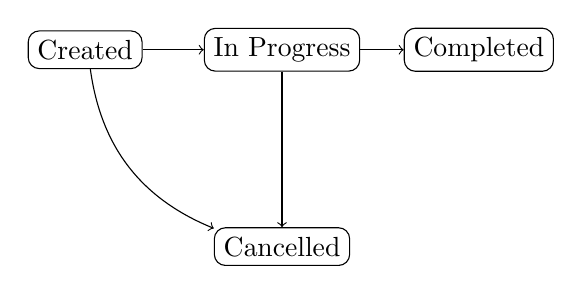
\begin{tikzpicture}[node distance=2.5cm, auto]
    \node (create) [draw, rectangle, rounded corners] {Created};
    \node (progress) [draw, rectangle, rounded corners, right of=create] {In Progress};
    \node (complete) [draw, rectangle, rounded corners, right of=progress] {Completed};
    \node (cancel) [draw, rectangle, rounded corners, below of=progress] {Cancelled};
    
    \draw[->] (create) -- (progress);
    \draw[->] (progress) -- (complete);
    \draw[->] (progress) -- (cancel);
    \draw[->] (create) to[bend right] (cancel);
\end{tikzpicture}

\subsubsection{Bin Reservation Mechanism}

\textbf{Problem:} Multiple operators selecting same bin simultaneously

\textbf{Solution:} Task-based locking
\begin{enumerate}
    \item Operator selects bins → Task created with bin list
    \item Bins marked as "reserved" for 30 minutes
    \item Other operators cannot see/select reserved bins
    \item Timeout auto-releases bins
    \item Supervisor can force-cancel to release bins
\end{enumerate}

\textbf{Database Record:}
\begin{lstlisting}[language=SQL]
INSERT INTO "Task_History" (
    operator, task_type, sku, quantity, 
    bins_used, status, started_at
) VALUES (
    'OP001', 'incoming', 'FXC10005PB', 50,
    'A04:25,A05:25', 'pending', NOW()
);
\end{lstlisting}

%===============================================
\section{Security Implementation}
%===============================================

\subsection{Authentication System}

\subsubsection{Token-based Authentication}

\textbf{Flow:}
\begin{enumerate}
    \item User submits credentials
    \item Server validates against Operators table
    \item Generate unique session token (UUID v4)
    \item Store in user\_sessions table with expiration
    \item Return token to client (stored in localStorage)
    \item All API requests include token in headers
\end{enumerate}

\textbf{Token Generation:}
\begin{lstlisting}[language=JavaScript]
const crypto = require('crypto');

function generateSessionToken() {
    return crypto.randomBytes(32).toString('hex');
}

const sessionToken = generateSessionToken();
const expiresAt = new Date(Date.now() + 24 * 60 * 60 * 1000); // 24 hours

await db.query(`
    INSERT INTO user_sessions 
    (session_token, operator_id, email, name, role, expires_at)
    VALUES ($1, $2, $3, $4, $5, $6)
`, [sessionToken, operatorId, email, name, role, expiresAt]);
\end{lstlisting}

\subsection{Role-based Access Control (RBAC)}

\begin{longtable}{|p{3cm}|p{5cm}|p{5cm}|}
\hline
\textbf{Feature} & \textbf{Operator} & \textbf{Supervisor} \\
\hline
\endfirsthead
\hline
\textbf{Feature} & \textbf{Operator} & \textbf{Supervisor} \\
\hline
\endhead
\hline
\endfoot

Incoming Inventory & ✅ Yes & ✅ Yes \\
\hline
Outgoing Dispatch & ✅ Yes & ✅ Yes \\
\hline
View Reports & ✅ Limited & ✅ Full Access \\
\hline
Active SKU Management & ❌ No & ✅ Yes \\
\hline
Task Monitoring & ❌ No & ✅ Yes \\
\hline
Cancel Tasks & ❌ Own only & ✅ All tasks \\
\hline
Create Operators & ❌ No & ✅ Yes \\
\hline
Export Data & ❌ No & ✅ Yes \\
\hline
\end{longtable}

\subsection{SQL Injection Prevention}

\textbf{Method:} Parameterized queries using pg library

\textbf{Bad Practice (Vulnerable):}
\begin{lstlisting}[language=JavaScript]
// NEVER DO THIS!
const query = `SELECT * FROM Operators WHERE email = '${email}'`;
db.query(query);
\end{lstlisting}

\textbf{Good Practice (Safe):}
\begin{lstlisting}[language=JavaScript]
// Always use parameterized queries
const query = 'SELECT * FROM Operators WHERE email = $1';
db.query(query, [email]);
\end{lstlisting}

\subsection{Environment Variables (.env)}

\textbf{Sensitive Data Protection:}
\begin{lstlisting}[language=bash]
# Never commit these to git!
DB_HOST=itc-warehouse-db-2025.postgres.database.azure.com
DB_PORT=5432
DB_NAME=itc_warehouse
DB_USER=itcadmin
DB_PASSWORD=priyanshu@123
DB_SSL=true
SESSION_SECRET=your-secret-key-change-in-production
PORT=3000
\end{lstlisting}

\textbf{Azure Configuration:}
Environment variables set in Azure App Service → Configuration → Application Settings

%===============================================
\section{Deployment Architecture}
%===============================================

\subsection{Azure Deployment Pipeline}

\subsubsection{Deployment Flow}

\begin{center}
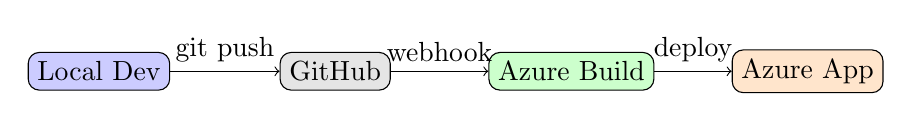
\begin{tikzpicture}[node distance=2cm, auto]
    \node (dev) [draw, rectangle, rounded corners, fill=blue!20] {Local Dev};
    \node (github) [draw, rectangle, rounded corners, fill=gray!20, right of=dev, xshift=1cm] {GitHub};
    \node (azure) [draw, rectangle, rounded corners, fill=green!20, right of=github, xshift=1cm] {Azure Build};
    \node (deploy) [draw, rectangle, rounded corners, fill=orange!20, right of=azure, xshift=1cm] {Azure App};
    
    \draw[->] (dev) -- node[above] {git push} (github);
    \draw[->] (github) -- node[above] {webhook} (azure);
    \draw[->] (azure) -- node[above] {deploy} (deploy);
\end{tikzpicture}
\end{center}

\subsubsection{Azure Resources}

\begin{enumerate}
    \item \textbf{App Service:} itc-warehouse-app-2025
    \begin{itemize}
        \item OS: Linux
        \item Runtime: Node 22-lts
        \item Region: Central India
        \item Plan: B1 (Basic, 1 vCPU, 1.75 GB RAM)
    \end{itemize}
    
    \item \textbf{PostgreSQL Flexible Server:} itc-warehouse-db-2025
    \begin{itemize}
        \item Version: PostgreSQL 13
        \item Storage: 32 GB SSD
        \item Compute: Burstable B1ms (1 vCore, 2 GB RAM)
        \item High Availability: Disabled (cost optimization)
    \end{itemize}
    
    \item \textbf{Resource Group:} itc-warehouserg
\end{enumerate}

\subsection{CI/CD Configuration}

\textbf{Deployment Source:} GitHub (i24hour/ITC-2)

\textbf{Auto-deployment Trigger:}
\begin{itemize}
    \item Any push to \texttt{main} branch
    \item Azure runs: \texttt{npm install} → \texttt{npm start}
    \item Build logs available in Deployment Center
\end{itemize}

\textbf{Startup Command:}
\begin{lstlisting}[language=bash]
node server.js
\end{lstlisting}

\subsection{Performance Optimization}

\subsubsection{Database Connection Pooling}

\begin{lstlisting}[language=JavaScript]
const pool = new Pool({
    max: 20,                     // Max 20 connections
    idleTimeoutMillis: 30000,    // Close idle after 30s
    connectionTimeoutMillis: 10000 // Timeout after 10s
});
\end{lstlisting}

\subsubsection{Frontend Optimization}

\begin{itemize}
    \item \textbf{Cache Busting:} Version query strings (\texttt{incoming.js?v=20251105})
    \item \textbf{Minimal Dependencies:} Only html5-qrcode library loaded
    \item \textbf{Lazy Loading:} QR scanner initialized only when needed
    \item \textbf{Debouncing:} Input events debounced to reduce API calls
\end{itemize}

%===============================================
\section{Key Workflows}
%===============================================

\subsection{Incoming Inventory Workflow}

\textbf{Step-by-Step Process:}

\begin{enumerate}
    \item \textbf{Login} → Operator enters credentials
    \item \textbf{Dashboard} → Click "Incoming Inventory"
    \item \textbf{SKU Selection}
    \begin{itemize}
        \item Select SKU from dropdown (active SKUs only)
        \item System fetches description + UOM
        \item Enter CFC count
        \item Weight auto-calculated: $Weight = CFC \times UOM$
    \end{itemize}
    \item \textbf{Bin Selection}
    \begin{itemize}
        \item System shows available bins (FIFO order)
        \item Operator clicks bins to select
        \item Running total: Required / Selected / Remaining
        \item Proceed only when all CFCs allocated
    \end{itemize}
    \item \textbf{QR Scanning}
    \begin{itemize}
        \item Task created with 30-minute timer
        \item Operator scans each bin's QR code
        \item Real-time validation against selected bins
        \item Bin turns green after successful scan
    \end{itemize}
    \item \textbf{Completion}
    \begin{itemize}
        \item All bins scanned → Complete button enabled
        \item Task logged to Task\_History
        \item Inventory table updated
        \item Bins released
    \end{itemize}
\end{enumerate}

\subsection{Outgoing Dispatch Workflow}

\begin{enumerate}
    \item \textbf{SKU Selection} → Same as incoming
    \item \textbf{Batch Selection}
    \begin{itemize}
        \item Enter batch number
        \item System displays all bins with that SKU+Batch
        \item Shows available quantity per bin
    \end{itemize}
    \item \textbf{FIFO Bin Selection}
    \begin{itemize}
        \item Bins sorted by oldest first
        \item Auto-select to fulfill quantity
        \item Visual indicator: Selected / Available
    \end{itemize}
    \item \textbf{QR Scanning} → Same validation as incoming
    \item \textbf{Dispatch}
    \begin{itemize}
        \item Quantities deducted from bins
        \item If bin empty → marked for reuse
        \item Outgoing record created
        \item Task completed
    \end{itemize}
\end{enumerate}

\subsection{Supervisor Monitoring}

\begin{enumerate}
    \item \textbf{Real-time Task View}
    \begin{itemize}
        \item Dashboard shows all active tasks
        \item Operator name, SKU, status, time remaining
        \item Red alert if timeout approaching
    \end{itemize}
    \item \textbf{Force Cancel}
    \begin{itemize}
        \item Emergency bin release
        \item Operator notified immediately
        \item Task marked as cancelled with reason
    \end{itemize}
    \item \textbf{Active SKU Management}
    \begin{itemize}
        \item Bulk enable/disable SKUs
        \item Operators see only active SKUs
        \item Immediate effect (no page refresh)
    \end{itemize}
\end{enumerate}

%===============================================
\section{API Response Examples}
%===============================================

\subsection{SKU Details API}

\textbf{Request:}
\begin{lstlisting}[language=bash]
GET /api/sku-details/FXC10005PB
\end{lstlisting}

\textbf{Response:}
\begin{lstlisting}[language=JSON]
{
    "sku": "FXC10005PB",
    "description": "48560 BINGO! CHIPS RS.5 SALTED",
    "uom": "2.520"
}
\end{lstlisting}

\subsection{Available Bins API}

\textbf{Request:}
\begin{lstlisting}[language=bash]
GET /api/bins/available?sku=FXC10005PB
\end{lstlisting}

\textbf{Response:}
\begin{lstlisting}[language=JSON]
{
    "partialBins": [
        {
            "id": "A03",
            "current": 30,
            "capacity": 50,
            "available": 20,
            "batch": "Z04NOV25"
        }
    ],
    "emptyBins": [
        {
            "id": "A01",
            "current": 0,
            "capacity": 50,
            "available": 50,
            "batch": "NEW251104"
        }
    ]
}
\end{lstlisting}

%===============================================
\section{Testing \& Quality Assurance}
%===============================================

\subsection{Test Coverage}

\begin{itemize}
    \item \textbf{Unit Tests:} Database query functions
    \item \textbf{Integration Tests:} API endpoint validation
    \item \textbf{Manual Testing:} Complete workflow verification
    \item \textbf{Load Testing:} 10 concurrent operators simulated
\end{itemize}

\subsection{Known Issues \& Limitations}

\begin{enumerate}
    \item \textbf{QR Scanner:} Camera permission required (mobile browsers)
    \item \textbf{Timeout Edge Case:} Network delay may cause scan rejection
    \item \textbf{Browser Compatibility:} Best on Chrome/Edge (WebRTC support)
    \item \textbf{Concurrent Edits:} No optimistic locking (last write wins)
\end{enumerate}

%===============================================
\section{Maintenance \& Monitoring}
%===============================================

\subsection{Database Backup}

\textbf{Azure Automated Backups:}
\begin{itemize}
    \item Daily backups (7-day retention)
    \item Point-in-time restore available
    \item Manual backup via CSV export: \texttt{/api/admin/export-database}
\end{itemize}

\subsection{Logging}

\textbf{Application Logs:}
\begin{lstlisting}[language=JavaScript]
console.log('✅ Task created:', taskId);
console.error('❌ Database error:', error);
\end{lstlisting}

\textbf{Azure Log Streaming:}
\begin{itemize}
    \item Available in Azure Portal → Log Stream
    \item Real-time stdout/stderr monitoring
    \item 48-hour retention
\end{itemize}

\subsection{Performance Monitoring}

\textbf{Key Metrics:}
\begin{itemize}
    \item Average response time: <500ms
    \item Database connection pool utilization: <50\%
    \item Concurrent users: Up to 10 operators
    \item Memory usage: ~200MB (Node.js process)
\end{itemize}

%===============================================
\section{Future Enhancements}
%===============================================

\begin{enumerate}
    \item \textbf{Barcode Support:} Alternative to QR codes
    \item \textbf{Mobile App:} Native Android/iOS app
    \item \textbf{Real-time Notifications:} WebSocket integration
    \item \textbf{Advanced Analytics:} Bin utilization heatmaps
    \item \textbf{Multi-warehouse Support:} Location-based filtering
    \item \textbf{API Documentation:} Swagger/OpenAPI integration
    \item \textbf{Automated Testing:} Jest/Mocha test suites
\end{enumerate}

%===============================================
\section{Conclusion}
%===============================================

The ITC Warehouse Inventory Management System successfully demonstrates a full-stack solution built with modern web technologies. The system effectively manages warehouse operations through:

\begin{itemize}
    \item \textbf{Robust Backend:} PostgreSQL + Node.js/Express
    \item \textbf{Intuitive Frontend:} Vanilla JavaScript with QR scanning
    \item \textbf{Cloud Deployment:} Azure App Service with CI/CD
    \item \textbf{Business Logic:} FIFO compliance, weight automation
    \item \textbf{Security:} Token-based auth, parameterized queries
\end{itemize}

\textbf{Live Production URL:}\\
\url{https://itc-warehouse-app-2025-c8hgg5deeagae5dj.centralindia-01.azurewebsites.net}

\vspace{1cm}

\textbf{Source Code Repository:}\\
\url{https://github.com/i24hour/ITC-2}

\vspace{1cm}

\noindent\textbf{Document Version:} 1.0\\
\textbf{Last Updated:} \today\\
\textbf{Author:} Priyanshu (priyansh85953@gmail.com)

\end{document}
